\documentclass[acmtog, authorversion]{acmart}
\usepackage[htt]{hyphenat}
\usepackage{graphicx}
\usepackage{lipsum}
\usepackage{pgfgantt}
\usepackage{enumitem}
\usepackage{booktabs}

\newlist{questions}{enumerate}{2}
\setlist[questions,1]{label=\textbf{RQ\arabic*.},ref=RQ\arabic*}
\setlist[questions,2]{label=(\alph*),ref=\thequestionsi(\alph*)}
\graphicspath{{images/}}

\AtBeginDocument{%
  \providecommand\BibTeX{{%
    \normalfont B\kern-0.5em{\scshape i\kern-0.25em b}\kern-0.8em\TeX}}}

\setcopyright{acmcopyright}
\copyrightyear{2023}
\acmYear{2023}

\acmConference[TScIT 39]{39$^{th}$ Twente Student Conference on IT}{July 8,
  2023}{Enschede, The Netherlands}

\begin{document}

\title{Satellite to Radar: Sequence to Sequence Learning for precipitation nowcasting}

\author{Mark Bruderer}
\email{m.a.bruderervanblerk@student.utwente.nl}
\affiliation{%
  \institution{University of Twente}
  \streetaddress{P.O. Box 217}
  \city{Enschede}
  \country{The Netherlands}
  \postcode{7500AE}
}

\renewcommand{\shortauthors}{Mark Bruderer}

\begin{abstract}
\section*{Abstract}
In this study we present \textbf{SatToRad} a sequence to sequence machine learning model capable of predicting radar reflectivity for lead times of 15, 30, 45, 60, 90 and 180 minutes.
\end{abstract}

\keywords{Machine Learning, Sequence to Sequence, Radar, Satellite, Storms, Forecasting}

\settopmatter{printacmref=false}

\begin{teaserfigure}
  \includegraphics*[width=\textwidth, trim= 0in 0.0in 0in 16.0in]{images/lightning.jpg}
  \caption{A supercell thunderstorm at twilight in SW Oklahoma.^1}
  \Description{A supercell thunderstorm at twilight in SW Oklahoma.}
  \label{fig:teaser}
\end{teaserfigure}

\maketitle

\section{Introduction}

Precipitation forecasting is essential to reduce the risk of life threatening situations. Different types of rainfall ranging from mist to heavy rain have a major impact for different societal sectors including agriculture, aviation, outdoor events, and the energy industry.
By having timely and accurate predictions of rainfall which in turn indicate the potential for destructive storms we can prevent injuries, assist companies in predicting energy production and use resources efficiently.
\medskip

% Predicting and understanding weather has become crucial in a number of industries, including agriculture, autonomous driving, aviation, or the energy sector. For example, weather conditions play a significant role for aviation and logistics companies in planning the fastest and safest route. Similarly, renewable energy companies need to be able to predict the amount of energy they will produce at a given day. As a consequence various weather models have been developed and are being applied all over the world. Unfortunately, these models often require highly specific information about the atmosphere and exact conditions.

% explain what storms are:
% - why are storms important
% - what are storms => how they from
A particularly strong threat is posed by rain storms and thunderstorms. Storms are one of the most destructive weather events in nature, capable of destroying human structures and even lead to loss of life \cite{noaa-national-severe-storms-laboratory-no-date}. Predicting storms is crucial and presents it's own set of challenges.
\medskip

% explain how to currently predict storms
At present meteorologists are able to successfully predict many instances of precipitation. Techniques that are used in practice range from manual analysis of current weather data (e.g radar or satellite images) to complex physics based simulations of our atmosphere with Numerical Weather Prediction (\textsc{NWP}) models.
\textsc{NWP} models predict precipitation based on \textit{optical flow}. Optical flow functions in two steps, first cumulonimbus clouds are identified, and then their movement is tracked to predict the location of precipitation. Thus in the case of \textsc{NWP} models, the \textit{cell-lifecycle} \cite{noaas-national-weather-service-no-date} is not taken into account \cite{prudden2020review}.
\medskip

% explain machine learning approaches
Machine Learning (\textsc{ML}) approaches have also been developed to predict precipitation. An improvement of machine learning models over \textsc{NWP} models is that they are much faster to produce predictions, thus ML models are more suitable for real-time or near-real-time predictions, such as required in disaster response and energy management. According to the universal approximation theorem \cite{cybenko-1989}, deep neural networks have the property of being able to approximate any function provided they have the correct weights, as such it is suggested that machine learning models can incorporate sources of predictability beyond optical flow such as the cell-lifecycle among others \cite{prudden2020review}.
\medskip

% explain our approach
Thus far most machine learning approaches for precipitation nowcasting have focused on predicting a next frame in a time series of radar reflectivity data \cite{shi2017deep, convlstm, rainet}. However taking this approach may eliminate the possibility of learning the cell-lifecycle, due to the fact that the model only sees precipitation itself but not the cloud that is causing the precipitation.
\medskip

% "Yet the key issue of precipitation prediction – the anticipation of convective initialization, as well as the growth and dissipation of precipitation in the imminent future – still appears to be unresolved" 

We propose to use multi-spectral satellite data to learn spatio-temporal mappings between sequences of satellite data and precipitation data. If this is successful cumulonimbus clouds could be predicted from when they are mere cumulus clouds and prior. An additional advantage is that satellite data as opposed to radar data is readily available over oceans and remote communities which allows for the prediction of precipitation over these regions. We will work towards creating a model by answering the following main research question:
\smallskip

% Most physical models are based on the extrapolation of the detected Cbs with atmospheric motion vectors (AMV; see [14] and the references therein). This approach works well as long as the cells do not decay during the prediction period. Unfortunately, cells usually do decay after a certain lifetime, such that this effect occurs regularly. Further, newly developed cells cannot be captured by extrapolation of detected cells. These are serious drawbacks of the AMV approach. The quite good results achieved with deep learning indicate that the training process might enable the network to gain information on the life cycles of cells (decay, newly developed cells). The network seems to be able to learn to a certain extent whether Cbs decay or newly develop within the prediction period or not, and we believe this is crucial for lead times around or larger than 180 min, as the lifetime of regular Cbs is usually shorter than this; see, e.g., 
% - 

% Radar has been the primary tool for predicting precipitation for decades, but it has limitations, such as its limited range and the fact that it cannot penetrate through heavy precipitation. This makes it difficult to predict precipitation in areas that are far from the radar, such as remote regions and over the ocean.

% Satellite data, on the other hand, can provide a global view of weather patterns and can be used to fill in gaps in radar coverage. Satellites can also provide information about cloud temperature, humidity, and other atmospheric conditions that can be used to infer the presence of precipitation. Additionally, satellite data can be useful for predicting the onset and duration of precipitation events, which can be valuable information for planning and emergency response.

% However, using satellite data for precipitation nowcasting also presents some challenges, such as the need to develop accurate algorithms for translating satellite data into precipitation estimates. These algorithms must take into account factors such as the altitude of the clouds, the types of precipitation (e.g. rain, snow, or hail), and the intensity of the precipitation. Despite these challenges, the use of satellite data for precipitation nowcasting shows great promise and has the potential to improve our ability to predict precipitation in a variety of settings.

\textbf{RQ1}: \textit{How can a deep learning model be trained to predict radar data with multi-spectral satellite data ?}
\smallskip

This research question will be answered by looking at the following sub research questions:
\begin{enumerate}
    \item \textit{what is necessary to build a well performing model ?}
    \item \textit{what methods can be used to create this model ?}
    \item \textit{what is the effectiveness of the trained model ?}
    \item \textit{what are the conditions under which the model can and cannot be used ?}
\end{enumerate}

\section{Main Contribution}
This proposal has the potential to contribute a model capable of predicting precipitation in the near future.

\section{Related Works}

In this section we will discuss the existing work in precipitation nowcasting via machine learning. This section is structured by the type of input data used in the approaches first we list radar based learning and then we discuss satellite based approaches.

\subsection{Radar Based Nowcasting}

Recurrent neural networks (\textsc{RNNs}) have been created to learn temporal relationships in data, therefore they are a natural candidate to the task of learning spatio-temporal patterns of weather. The \textsc{LSTM} architecture was developed by Hochreiter and Schmidhuber \cite{lstm}, to solve the problem of vanishing and exploding gradients in RNNs and is widely used. Taking LSTM as a base and adapting the weights to kernels, \textsc{ConvLSTM} \cite{convlstm} was introduced in 2015 for the task of precipitation forecasting. Multiple layers of ConvLSTM are used in this paper to obtain a sequence to sequence architecture. A further improvement of ConvLSTM is \textsc{trajGRU} which was proposed by Shi et al. \cite{shi2017deep} to be able to learn \textit{location-variant} structure for recurrent connections.
\medskip

Simple convolutional neural networks have also been used to predict precipitation. As demonstrated by Bai et al. and Gering et al. \cite{bai2018empirical, gehring2017convolutional} convolutional neural architectures can outperform recurrent neural networks for a variety of sequence modelling tasks. This is the reason why many works on precipitation nowcasting have used pure convolutional networks \cite{rainet,agrawal2019machine}
\medskip

Due to machine learning models attempting to minimize loss, blurry predictions can be produced by models. This can be alleviated by using generative models which sample from the possible futures. Generative models have been succesfully applied to the task of precipitation nowcasting \cite{}.

% Instead of treating the problem as a spatio temporal problem others have treated the problem as a image translation problem. using UNEt
% One possible approach to forecast precipitation is through the use of convolutional neural networks such as U-NET proposed by Ronneberger et al. for image segmentation \cite{ronneberger2015unet}

\begin{enumerate}
    \item convolutional neural networks
    \item recurrent neural networks
    \item generative adverserial networks
    \item variational autoencoders
\end{enumerate}

\subsection{Satellite Based Nowcasting}

\begin{enumerate}
    \item multi layer perceptron
    \item convolutional neural networks (u-net)
\end{enumerate}

% In their 2019 paper a Multi Layer Perceptron network was used to estimate precipitation data via satellite channels. \cite{precipitationEstimationFromSat}

% In the blog post \cite{wirth-2022} a U-Net network was used to predict precipitation data based on satellite data.

% In both of these approaches only data provenant from the infrared channels was used.

% A related approach is that of \cite{predictionLightning}
% which does not predict precipitation directly but uses lightning as a marker for storms. This paper uses a U-Net architecture to predict triangulated lightning events from satellite images. This paper provides the contribution that they observed in their model that both the visual channels and the infrared channels of the satellite provide sources of predicatability and can both be leveraged to produce good predictions.






























% To read a comprehensive literature review of the available work in radar nowcasting see \cite{prudden2020review}. 

% Since in our approach we Problem can be approached as a video prediction problem. It is more suitable to approximate the problem to an sequence to sequence learning problem, where sequences from the domain of satellite images in the past need to be converted into the the domain of radar data.

% The first paper to forecast precipitation via machine learning was \cite{}. Convolutional LSTM a machine was proposed for the application of solving the precipitation nowcasting problem in 2015.

% study \cite{nhess-22-577-2022} measured the importance of features for thunderstorm prediction, it found that satellite was the strongest feature, they suggest that satellite images are also valuable and can offer a good alternative for places with missing satellite data, like over oceans and less developed areas.

% Additionally data driven methods have been used to predict precipitation. Additionally various foundation models have been presented to be fine-tuned to solve meteorological tasks \cite{nguyen2023climax, bi2022panguweather}.

\section{Background}
In order to understand this research it is important to be acquainted with the machine learning techniques that will be used. Furthermore insight into this study can be enhanced by having more in depth information on the used data-sets and the meteorological theory.

MLP
Convolutional Neural Networks
RNNs
Sequence to sequence models

Serviri paper
Satellite paper
Cumulonimbus paper

\section{Methods}

% Can also be a new way to solve the problem or a hybrid method (mixed strategy, etc..). In this case, it would be nice to see a description of the steps which are followed in order to solve the problem.

In this section we will discuss how we will approach the problem of precipitation nowcasting. As previously mentioned we will focus on the prediction of radar reflectivity by using satellite data. Radar reflectivity can be converted to precipitation (in mm per hour) by using the Marshall-Palmer formula.

$$R = (\frac{10^{dbZ/10}}{200})^{\frac{5}{8}}$$

Practically we will perform this with the following methods:
\begin{enumerate}
    \item Data Preprocessing
    \item Model Training
    \item Model Evaluation
\end{enumerate}

\subsection{Data Preprocessing}
The obtained satellite images are in \textit{Geostationary} projection, and provide a view of Eurasia and Africa. We will process this data by reprojecting the data into \textit{Mercator} projection. Furthermore we will zoom in to match the area captured in the radar images. Both of these steps will be performed by using the \texttt{satpy} package \cite{}.

Then satellite channels of the same timestamp will be aggregated into the channels dimension of the tensor.

Last dimension of the tensor will be the satellite channels instead of normal rgb.

\texttt{(timesteps, h, w, channels)}

output will be of shape \texttt{(timesteps, h, w)}

\subsection{Model Training}

\subsection{Model Evaluation}
Expert based evaluation and month study.

\section{Expected Results}

\subsection{Data}

We have obtained a multi-year structured archive of radar composites with a temporal resolution of 5 minutes. These radar composites are made from 5 Doppler radars that provide a good coverage of the Benelux area, these radars are located at these points and can be visualized in figure \ref{}
\begin{itemize}
    \item \textsc{Den Helder}
    \item \textsc{Herwijnen}
    \item \textsc{Essen}
    \item \textsc{Borkum}
    \item \textsc{Neuheilenbach}
\end{itemize}


Additionally we have obtained satellite data from \textsc{EUMETSAT} at a 3x3km spatial resoulution and 15 minute temporal resolution. This data has been captured with the \textsc{SEVIRI} sensor, which produces multichannel satellite imagery.

\begin{figure}
    \centering
    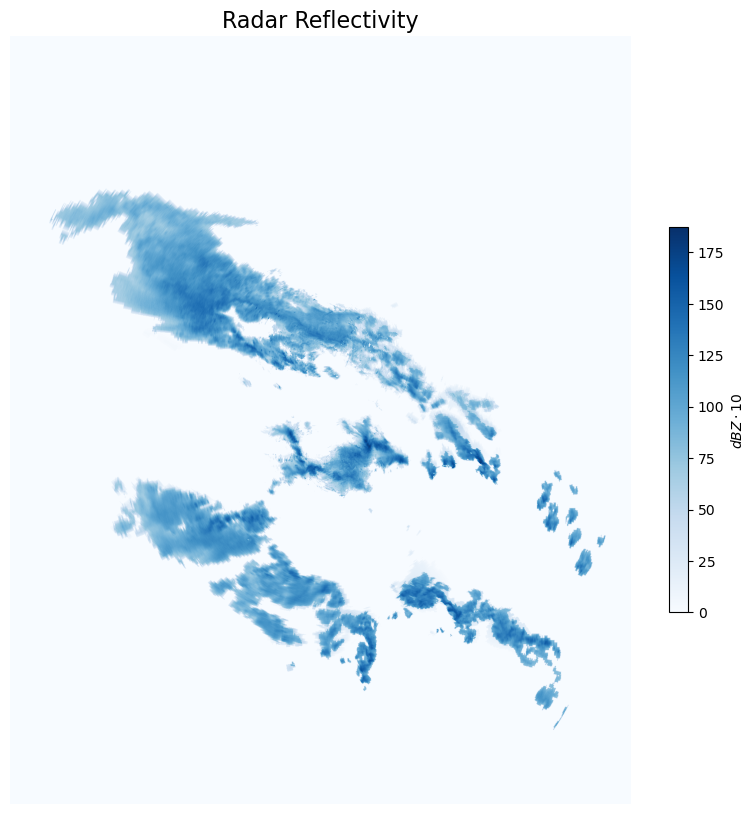
\includegraphics[width=225]{report/images/radar_reflectivity.png}
    \caption{Radar Reflectivity}
    \label{fig:my_label}
\end{figure}

\begin{figure}
    \centering
    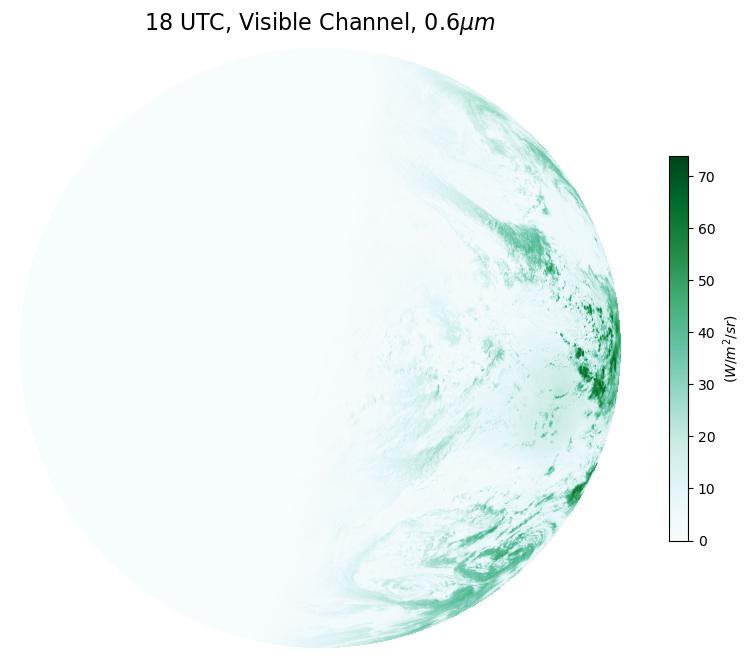
\includegraphics[width=225]{report/images/vis_006.png}
    \caption{Satellite Image: Visible Channel 18UTC 0.6\mu m}
    \label{fig:my_label}
\end{figure}

\begin{figure}
    \centering
    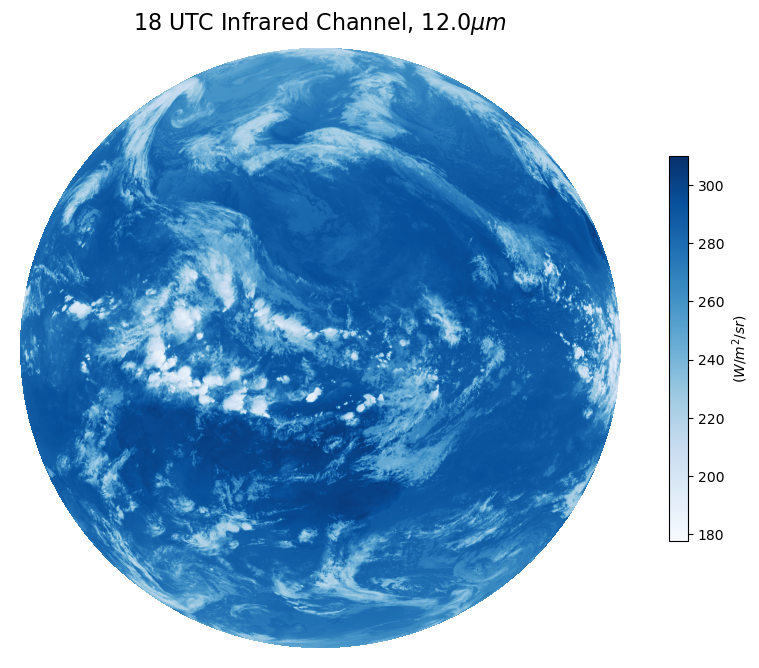
\includegraphics[width=225]{report/images/infrared.png}
    \caption{Satellite Image: Infrared Channel 18UTC 12.0\mu m}
    \label{fig:my_label}
\end{figure}

\subsection{Implementation Details}

\subsection{Metrics}

\begin{enumerate}
    \item MSE
    \item MAE
    \item RMSE
    \item B-MSE
    \item B-MAE
    \item CSI
\end{enumerate}

exteded to perceptual and other content losses originating from superzoom studies.

\subsection{Experiments}


\section{Time Planning}
In this section we discuss our planning for the execution of the study in this proposal. In figure \ref{}

\medskip

\begin{ganttchart}[hgrid,vgrid,
bar/.append style={fill=blue!50},
group/.append style={draw=black, fill=gray!50},
milestone/.append style={fill=yellow!50, rounded corners=3pt}]{1}{11}
  \gantttitle{\textbf{Planning Table}}{11} \\
  \gantttitlelist{1,...,11}{1} \\
  \ganttgroup{Research}{1}{11} \\
  \ganttbar{Proposal}{1}{2} \\
  \ganttmilestone{Draft Proposal}{2} \\
  \ganttmilestone{Final Proposal}{3} \\
  \ganttbar{Writing}{3}{10} \\
  % \ganttlinkedbar{Task 2}{3}{8} \ganttnewline
  % \ganttbar{Final Task}{8}{12} \\
  \ganttmilestone{Draft Paper}{9} \\
  \ganttmilestone{Final Paper}{10} \\
  \ganttbar{Presentation}{11}{11} \\
  \ganttlink{elem1}{elem4}
  \ganttgroup{Experiments}{1}{11} \\
  \ganttbar{Experiment 1}{2}{4} \\
\end{ganttchart}


\section{Conclusions}



\begin{acks}
Infoplaza B.V
\end{acks}

\bibliographystyle{ACM-Reference-Format}
\bibliography{ref}

\appendix
%Appendix A
\section{Headings in Appendices}
The rules about hierarchical headings discussed above for the body
of the article are different in the appendices. In the
\textbf{appendix} environment, the command \textbf{section} is
used to indicate the start of each Appendix, with alphabetic order
designation (i.e. the first is A, the second B, etc.) and a title
(if you include one). So, if you need hierarchical structure
\textit{within} an Appendix, start with \textbf{subsection} as the
highest level. Here is an outline of the body of this document in
Appendix-appropriate form:
\subsection{Appendix A.1}
Sample text.
\subsection{Appendix A.2}
Sample text.
\subsubsection{Appendix A.2.1}
Sample text.

\begin{table}[]
\caption{Reflectivity in dBZ versus Rainrate}
\begin{tabular}{@{}llll@{}}
\toprule
LZ(dBZ) & R(mm/h) & R(in/h)        & Intensity             \\ \midrule
5       & (mm/h)  & \textless 0.01 & Hardly noticeable     \\
10      & 0.15    & \textless 0.01 & Light mist            \\
15      & 0.3     & 0.01           & Mist                  \\
20      & 0.6     & 0.02           & Very light            \\
25      & 1.3     & 0.05           & Light                 \\
30      & 2.7     & 0.10           & Light to moderate     \\
35      & 5.6     & 0.22           & Moderate rain         \\
40      & 11.53   & 0.45           & Moderate rain         \\
45      & 23.7    & 0.92           & Moderate to heavy     \\
50      & 48.6    & 1.90           & Heavy                 \\
55      & 100     & 4              & Very heavy/small hail \\
60      & 205     & 8              & Extreme/moderate hail \\
65      & 421     & 16.6           & Extreme/large hail    \\ \bottomrule
\end{tabular}
\end{table}

\paragraph{Inline (In-text) Equations}
% This next section command marks the start of
% Appendix B, and does not continue the present hierarchy
\section{Appendix B}
Sample text.
%\balancecolumns % GM June 2007
% That's all folks!


\end{document}
\endinput
%%
%% End of file `sample-authordraft.tex'.
